% Options for packages loaded elsewhere
% Options for packages loaded elsewhere
\PassOptionsToPackage{unicode}{hyperref}
\PassOptionsToPackage{hyphens}{url}
\PassOptionsToPackage{dvipsnames,svgnames,x11names}{xcolor}
%
\documentclass[
  letterpaper,
  DIV=11,
  numbers=noendperiod]{scrartcl}
\usepackage{xcolor}
\usepackage{amsmath,amssymb}
\setcounter{secnumdepth}{2}
\usepackage{iftex}
\ifPDFTeX
  \usepackage[T1]{fontenc}
  \usepackage[utf8]{inputenc}
  \usepackage{textcomp} % provide euro and other symbols
\else % if luatex or xetex
  \usepackage{unicode-math} % this also loads fontspec
  \defaultfontfeatures{Scale=MatchLowercase}
  \defaultfontfeatures[\rmfamily]{Ligatures=TeX,Scale=1}
\fi
\usepackage{lmodern}
\ifPDFTeX\else
  % xetex/luatex font selection
\fi
% Use upquote if available, for straight quotes in verbatim environments
\IfFileExists{upquote.sty}{\usepackage{upquote}}{}
\IfFileExists{microtype.sty}{% use microtype if available
  \usepackage[]{microtype}
  \UseMicrotypeSet[protrusion]{basicmath} % disable protrusion for tt fonts
}{}
\makeatletter
\@ifundefined{KOMAClassName}{% if non-KOMA class
  \IfFileExists{parskip.sty}{%
    \usepackage{parskip}
  }{% else
    \setlength{\parindent}{0pt}
    \setlength{\parskip}{6pt plus 2pt minus 1pt}}
}{% if KOMA class
  \KOMAoptions{parskip=half}}
\makeatother
% Make \paragraph and \subparagraph free-standing
\makeatletter
\ifx\paragraph\undefined\else
  \let\oldparagraph\paragraph
  \renewcommand{\paragraph}{
    \@ifstar
      \xxxParagraphStar
      \xxxParagraphNoStar
  }
  \newcommand{\xxxParagraphStar}[1]{\oldparagraph*{#1}\mbox{}}
  \newcommand{\xxxParagraphNoStar}[1]{\oldparagraph{#1}\mbox{}}
\fi
\ifx\subparagraph\undefined\else
  \let\oldsubparagraph\subparagraph
  \renewcommand{\subparagraph}{
    \@ifstar
      \xxxSubParagraphStar
      \xxxSubParagraphNoStar
  }
  \newcommand{\xxxSubParagraphStar}[1]{\oldsubparagraph*{#1}\mbox{}}
  \newcommand{\xxxSubParagraphNoStar}[1]{\oldsubparagraph{#1}\mbox{}}
\fi
\makeatother

\usepackage{color}
\usepackage{fancyvrb}
\newcommand{\VerbBar}{|}
\newcommand{\VERB}{\Verb[commandchars=\\\{\}]}
\DefineVerbatimEnvironment{Highlighting}{Verbatim}{commandchars=\\\{\}}
% Add ',fontsize=\small' for more characters per line
\usepackage{framed}
\definecolor{shadecolor}{RGB}{241,243,245}
\newenvironment{Shaded}{\begin{snugshade}}{\end{snugshade}}
\newcommand{\AlertTok}[1]{\textcolor[rgb]{0.68,0.00,0.00}{#1}}
\newcommand{\AnnotationTok}[1]{\textcolor[rgb]{0.37,0.37,0.37}{#1}}
\newcommand{\AttributeTok}[1]{\textcolor[rgb]{0.40,0.45,0.13}{#1}}
\newcommand{\BaseNTok}[1]{\textcolor[rgb]{0.68,0.00,0.00}{#1}}
\newcommand{\BuiltInTok}[1]{\textcolor[rgb]{0.00,0.23,0.31}{#1}}
\newcommand{\CharTok}[1]{\textcolor[rgb]{0.13,0.47,0.30}{#1}}
\newcommand{\CommentTok}[1]{\textcolor[rgb]{0.37,0.37,0.37}{#1}}
\newcommand{\CommentVarTok}[1]{\textcolor[rgb]{0.37,0.37,0.37}{\textit{#1}}}
\newcommand{\ConstantTok}[1]{\textcolor[rgb]{0.56,0.35,0.01}{#1}}
\newcommand{\ControlFlowTok}[1]{\textcolor[rgb]{0.00,0.23,0.31}{\textbf{#1}}}
\newcommand{\DataTypeTok}[1]{\textcolor[rgb]{0.68,0.00,0.00}{#1}}
\newcommand{\DecValTok}[1]{\textcolor[rgb]{0.68,0.00,0.00}{#1}}
\newcommand{\DocumentationTok}[1]{\textcolor[rgb]{0.37,0.37,0.37}{\textit{#1}}}
\newcommand{\ErrorTok}[1]{\textcolor[rgb]{0.68,0.00,0.00}{#1}}
\newcommand{\ExtensionTok}[1]{\textcolor[rgb]{0.00,0.23,0.31}{#1}}
\newcommand{\FloatTok}[1]{\textcolor[rgb]{0.68,0.00,0.00}{#1}}
\newcommand{\FunctionTok}[1]{\textcolor[rgb]{0.28,0.35,0.67}{#1}}
\newcommand{\ImportTok}[1]{\textcolor[rgb]{0.00,0.46,0.62}{#1}}
\newcommand{\InformationTok}[1]{\textcolor[rgb]{0.37,0.37,0.37}{#1}}
\newcommand{\KeywordTok}[1]{\textcolor[rgb]{0.00,0.23,0.31}{\textbf{#1}}}
\newcommand{\NormalTok}[1]{\textcolor[rgb]{0.00,0.23,0.31}{#1}}
\newcommand{\OperatorTok}[1]{\textcolor[rgb]{0.37,0.37,0.37}{#1}}
\newcommand{\OtherTok}[1]{\textcolor[rgb]{0.00,0.23,0.31}{#1}}
\newcommand{\PreprocessorTok}[1]{\textcolor[rgb]{0.68,0.00,0.00}{#1}}
\newcommand{\RegionMarkerTok}[1]{\textcolor[rgb]{0.00,0.23,0.31}{#1}}
\newcommand{\SpecialCharTok}[1]{\textcolor[rgb]{0.37,0.37,0.37}{#1}}
\newcommand{\SpecialStringTok}[1]{\textcolor[rgb]{0.13,0.47,0.30}{#1}}
\newcommand{\StringTok}[1]{\textcolor[rgb]{0.13,0.47,0.30}{#1}}
\newcommand{\VariableTok}[1]{\textcolor[rgb]{0.07,0.07,0.07}{#1}}
\newcommand{\VerbatimStringTok}[1]{\textcolor[rgb]{0.13,0.47,0.30}{#1}}
\newcommand{\WarningTok}[1]{\textcolor[rgb]{0.37,0.37,0.37}{\textit{#1}}}

\usepackage{longtable,booktabs,array}
\usepackage{calc} % for calculating minipage widths
% Correct order of tables after \paragraph or \subparagraph
\usepackage{etoolbox}
\makeatletter
\patchcmd\longtable{\par}{\if@noskipsec\mbox{}\fi\par}{}{}
\makeatother
% Allow footnotes in longtable head/foot
\IfFileExists{footnotehyper.sty}{\usepackage{footnotehyper}}{\usepackage{footnote}}
\makesavenoteenv{longtable}
\usepackage{graphicx}
\makeatletter
\newsavebox\pandoc@box
\newcommand*\pandocbounded[1]{% scales image to fit in text height/width
  \sbox\pandoc@box{#1}%
  \Gscale@div\@tempa{\textheight}{\dimexpr\ht\pandoc@box+\dp\pandoc@box\relax}%
  \Gscale@div\@tempb{\linewidth}{\wd\pandoc@box}%
  \ifdim\@tempb\p@<\@tempa\p@\let\@tempa\@tempb\fi% select the smaller of both
  \ifdim\@tempa\p@<\p@\scalebox{\@tempa}{\usebox\pandoc@box}%
  \else\usebox{\pandoc@box}%
  \fi%
}
% Set default figure placement to htbp
\def\fps@figure{htbp}
\makeatother





\setlength{\emergencystretch}{3em} % prevent overfull lines

\providecommand{\tightlist}{%
  \setlength{\itemsep}{0pt}\setlength{\parskip}{0pt}}



 


\KOMAoption{captions}{tableheading}
\usepackage{marginnote, here, relsize, needspace, setspace} \def\it{\emph}
\makeatletter
\@ifpackageloaded{tcolorbox}{}{\usepackage[skins,breakable]{tcolorbox}}
\@ifpackageloaded{fontawesome5}{}{\usepackage{fontawesome5}}
\definecolor{quarto-callout-color}{HTML}{909090}
\definecolor{quarto-callout-note-color}{HTML}{0758E5}
\definecolor{quarto-callout-important-color}{HTML}{CC1914}
\definecolor{quarto-callout-warning-color}{HTML}{EB9113}
\definecolor{quarto-callout-tip-color}{HTML}{00A047}
\definecolor{quarto-callout-caution-color}{HTML}{FC5300}
\definecolor{quarto-callout-color-frame}{HTML}{acacac}
\definecolor{quarto-callout-note-color-frame}{HTML}{4582ec}
\definecolor{quarto-callout-important-color-frame}{HTML}{d9534f}
\definecolor{quarto-callout-warning-color-frame}{HTML}{f0ad4e}
\definecolor{quarto-callout-tip-color-frame}{HTML}{02b875}
\definecolor{quarto-callout-caution-color-frame}{HTML}{fd7e14}
\makeatother
\makeatletter
\@ifpackageloaded{caption}{}{\usepackage{caption}}
\AtBeginDocument{%
\ifdefined\contentsname
  \renewcommand*\contentsname{Table of contents}
\else
  \newcommand\contentsname{Table of contents}
\fi
\ifdefined\listfigurename
  \renewcommand*\listfigurename{List of Figures}
\else
  \newcommand\listfigurename{List of Figures}
\fi
\ifdefined\listtablename
  \renewcommand*\listtablename{List of Tables}
\else
  \newcommand\listtablename{List of Tables}
\fi
\ifdefined\figurename
  \renewcommand*\figurename{Figure}
\else
  \newcommand\figurename{Figure}
\fi
\ifdefined\tablename
  \renewcommand*\tablename{Table}
\else
  \newcommand\tablename{Table}
\fi
}
\@ifpackageloaded{float}{}{\usepackage{float}}
\floatstyle{ruled}
\@ifundefined{c@chapter}{\newfloat{codelisting}{h}{lop}}{\newfloat{codelisting}{h}{lop}[chapter]}
\floatname{codelisting}{Listing}
\newcommand*\listoflistings{\listof{codelisting}{List of Listings}}
\makeatother
\makeatletter
\makeatother
\makeatletter
\@ifpackageloaded{caption}{}{\usepackage{caption}}
\@ifpackageloaded{subcaption}{}{\usepackage{subcaption}}
\makeatother
\usepackage{bookmark}
\IfFileExists{xurl.sty}{\usepackage{xurl}}{} % add URL line breaks if available
\urlstyle{same}
\hypersetup{
  pdftitle={Lab 4 - Multinomial Regression},
  pdfauthor={Suyog Chandramouli},
  colorlinks=true,
  linkcolor={blue},
  filecolor={Maroon},
  citecolor={Blue},
  urlcolor={Blue},
  pdfcreator={LaTeX via pandoc}}


\title{Lab 4 - Multinomial Regression}
\author{Suyog Chandramouli}
\date{2026-03-07}
\begin{document}
\maketitle


\textbf{Lab Goal:} Predict voting frequency using demographic
variables\\
\textbf{Data source:} FiveThirtyEight ``Why Many Americans Don't Vote''
survey\\
\textbf{Method:} Multinomial logistic regression

\subsection{Instructions}\label{instructions}

\begin{itemize}
\tightlist
\item
  If you are fitting a model, display the model output in a neatly
  formatted table. (The \texttt{tidy()} and \texttt{kable()} functions
  can help!)
\item
  If you are creating a plot, use clear labels for all axes, titles,
  etc.
\item
  Commit and push your work to GitHub regularly, at least after each
  exercise. Write short and informative commit messages.
\item
  When you're done, we should be able to knit the final version of the
  QMD in your GitHub as an HTML.
\end{itemize}

\begin{tcolorbox}[enhanced jigsaw, toprule=.15mm, opacitybacktitle=0.6, coltitle=black, opacityback=0, bottomrule=.15mm, left=2mm, colframe=quarto-callout-tip-color-frame, leftrule=.75mm, toptitle=1mm, colbacktitle=quarto-callout-tip-color!10!white, rightrule=.15mm, colback=white, title=\textcolor{quarto-callout-tip-color}{\faLightbulb}\hspace{0.5em}{Workflow tip}, arc=.35mm, bottomtitle=1mm, titlerule=0mm, breakable]

Work through the lab by running chunks \textbf{one at a time} in RStudio
(Cmd/Ctrl + Enter), not by rendering the whole document. Render only at
the end, once all your code is working.

This is how most R users actually work -- you'd write a line, run it,
check the output, and iterate. Rendering is for producing the final
document. When you render, Quarto starts a fresh R session and runs
every chunk top-to-bottom, so if anything is incomplete, everything
downstream breaks. When you work interactively using chunks, your
environment builds up as you go, so you always have your objects
available to inspect and troubleshoot.

The \textbf{``Run All Chunks Above''} button (downward arrow with a bar,
next to the green play button in each chunk) is another useful tool. It
re-runs everything from the top of the document up to your current
chunk, so all your objects are up to date before you start working on
the next question.

\end{tcolorbox}

\subsection{Setup}\label{setup}

\begin{Shaded}
\begin{Highlighting}[]
\FunctionTok{library}\NormalTok{(nnet)}
\FunctionTok{library}\NormalTok{(car)}
\FunctionTok{library}\NormalTok{(tidyverse)}
\FunctionTok{library}\NormalTok{(emmeans)}
\FunctionTok{library}\NormalTok{(ggeffects)}
\FunctionTok{library}\NormalTok{(knitr)}
\FunctionTok{library}\NormalTok{(patchwork)}
\FunctionTok{library}\NormalTok{(broom)}
\FunctionTok{library}\NormalTok{(parameters)}
\FunctionTok{library}\NormalTok{(easystats)}
\FunctionTok{library}\NormalTok{(viridis)}
\end{Highlighting}
\end{Shaded}

\begin{center}\rule{0.5\linewidth}{0.5pt}\end{center}

\section{Part 1: Data Preparation}\label{part-1-data-preparation}

\subsection{The Data}\label{the-data}

The data for this assignment comes from an online Ipsos survey that was
conducted for the FiveThirtyEight article
\href{https://projects.fivethirtyeight.com/non-voters-poll-2020-election/}{``Why
Many Americans Don't Vote''}. If you'd like, you can read more about the
survey design and respondents in the README of the
\href{https://github.com/fivethirtyeight/data/tree/master/non-voters}{GitHub
repo} for the data, but all the necessary information is explained
below.

Respondents were asked a variety of questions about their political
beliefs, thoughts on multiple issues, and voting behavior. We will focus
on using the demographic variables and someone's party identification to
understand whether a person is a probable voter.

The variables we'll focus on are (definitions from the codebook in data
set GitHub repo):

\begin{itemize}
\item
  \texttt{ppage}: Age of respondent
\item
  \texttt{educ}: Highest educational attainment category
\item
  \texttt{race}: Race of respondent, census categories. Note: all
  categories except Hispanic were non-Hispanic.
\item
  \texttt{gender}: Gender of respondent
\item
  \texttt{income\_cat}: Household income category of respondent
\item
  \texttt{Q30}: Response to the question ``Generally speaking, do you
  think of yourself as a\ldots{}''

  \begin{itemize}
  \tightlist
  \item
    1: Republican
  \item
    2: Democrat
  \item
    3: Independent
  \item
    4: Another party, please specify
  \item
    5: No preference
  \item
    -1: No response
  \end{itemize}
\item
  \texttt{voter\_category}: past voting behavior:

  \begin{itemize}
  \tightlist
  \item
    \textbf{always}: respondent voted in all or all-but-one of the
    elections they were eligible in
  \item
    \textbf{sporadic}: respondent voted in at least two, but fewer than
    all-but-one of the elections they were eligible in
  \item
    \textbf{rarely/never}: respondent voted in 0 or 1 of the elections
    they were eligible in
  \end{itemize}
\end{itemize}

\begin{Shaded}
\begin{Highlighting}[]
\NormalTok{voter\_data }\OtherTok{\textless{}{-}} \FunctionTok{read\_csv}\NormalTok{(}\StringTok{"https://raw.githubusercontent.com/fivethirtyeight/data/master/non{-}voters/nonvoters\_data.csv"}\NormalTok{)}
\end{Highlighting}
\end{Shaded}

The variable \texttt{Q30} contains the respondent's political party
identification. The following code simplifies \texttt{Q30} into four
categories:

\begin{Shaded}
\begin{Highlighting}[]
\NormalTok{voter\_data }\OtherTok{\textless{}{-}}\NormalTok{ voter\_data }\SpecialCharTok{\%\textgreater{}\%}
  \FunctionTok{mutate}\NormalTok{(}\AttributeTok{pol\_ident =} \FunctionTok{case\_when}\NormalTok{(}
\NormalTok{    Q30 }\SpecialCharTok{==} \DecValTok{1} \SpecialCharTok{\textasciitilde{}} \StringTok{"Rep"}\NormalTok{,}
\NormalTok{    Q30 }\SpecialCharTok{==} \DecValTok{2} \SpecialCharTok{\textasciitilde{}} \StringTok{"Dem"}\NormalTok{,}
\NormalTok{    Q30 }\SpecialCharTok{==} \DecValTok{3} \SpecialCharTok{\textasciitilde{}} \StringTok{"Indep"}\NormalTok{,}
    \ConstantTok{TRUE} \SpecialCharTok{\textasciitilde{}} \StringTok{"Other"}
\NormalTok{  ))}
\NormalTok{voter\_data}
\end{Highlighting}
\end{Shaded}

\begin{verbatim}
# A tibble: 5,836 x 120
   RespId weight    Q1  Q2_1  Q2_2  Q2_3  Q2_4  Q2_5  Q2_6  Q2_7  Q2_8  Q2_9
    <dbl>  <dbl> <dbl> <dbl> <dbl> <dbl> <dbl> <dbl> <dbl> <dbl> <dbl> <dbl>
 1 470001  0.752     1     1     1     2     4     1     4     2     2     4
 2 470002  1.03      1     1     2     2     3     1     1     2     1     1
 3 470003  1.08      1     1     1     2     2     1     1     2     1     4
 4 470007  0.682     1     1     1     1     3     1     1     1     1     1
 5 480008  0.991     1     1     1    -1     1     1     1     1     1     1
 6 480009  1.06      1     3     2     3     4     1     3     3     1     1
 7 480010  1.15      1     1     1     2     3     1     1     1     1     1
 8 470008  1.02      1     1     1     2     2     1     3     1     1     4
 9 470010  0.818     1     1     1     1     3     1     1     1     1     3
10 470011  1.17      1     1     1     2     1     1     1     1     2     1
# i 5,826 more rows
# i 108 more variables: Q2_10 <dbl>, Q3_1 <dbl>, Q3_2 <dbl>, Q3_3 <dbl>,
#   Q3_4 <dbl>, Q3_5 <dbl>, Q3_6 <dbl>, Q4_1 <dbl>, Q4_2 <dbl>, Q4_3 <dbl>,
#   Q4_4 <dbl>, Q4_5 <dbl>, Q4_6 <dbl>, Q5 <dbl>, Q6 <dbl>, Q7 <dbl>,
#   Q8_1 <dbl>, Q8_2 <dbl>, Q8_3 <dbl>, Q8_4 <dbl>, Q8_5 <dbl>, Q8_6 <dbl>,
#   Q8_7 <dbl>, Q8_8 <dbl>, Q8_9 <dbl>, Q9_1 <dbl>, Q9_2 <dbl>, Q9_3 <dbl>,
#   Q9_4 <dbl>, Q10_1 <dbl>, Q10_2 <dbl>, Q10_3 <dbl>, Q10_4 <dbl>, ...
\end{verbatim}

\subsubsection*{Question 1.1}\label{question-1.1}
\addcontentsline{toc}{subsubsection}{Question 1.1}

The variable \texttt{voter\_category} identifies the respondent's past
voter behavior. Relevel the variable to make \textbf{rarely/never} the
baseline level, followed by sporadic, then always.

\begin{tcolorbox}[enhanced jigsaw, toprule=.15mm, opacitybacktitle=0.6, coltitle=black, opacityback=0, bottomrule=.15mm, left=2mm, colframe=quarto-callout-tip-color-frame, leftrule=.75mm, toptitle=1mm, colbacktitle=quarto-callout-tip-color!10!white, rightrule=.15mm, colback=white, title=\textcolor{quarto-callout-tip-color}{\faLightbulb}\hspace{0.5em}{Hint}, arc=.35mm, bottomtitle=1mm, titlerule=0mm, breakable]

Use \texttt{factor()} with the \texttt{levels} argument to set the
ordering. The first level becomes the baseline in \texttt{multinom()}.

\end{tcolorbox}

\begin{Shaded}
\begin{Highlighting}[]
\CommentTok{\# Enter your code}
\NormalTok{voter\_data}\SpecialCharTok{$}\NormalTok{voter\_category }\OtherTok{\textless{}{-}} \FunctionTok{factor}\NormalTok{(voter\_data}\SpecialCharTok{$}\NormalTok{voter\_category, }
                \AttributeTok{levels =} \FunctionTok{c}\NormalTok{(}\StringTok{"rarely/never"}\NormalTok{, }\StringTok{"sporadic"}\NormalTok{, }\StringTok{"always"}\NormalTok{), }
                \AttributeTok{ordered =} \ConstantTok{TRUE}\NormalTok{)}
\end{Highlighting}
\end{Shaded}

\subsubsection*{Question 1.2}\label{question-1.2}
\addcontentsline{toc}{subsubsection}{Question 1.2}

Mean-center the age variable (\texttt{ppage}) so that the intercept
reflects the log-odds for an average-aged person rather than a
0-year-old.

\begin{Shaded}
\begin{Highlighting}[]
\CommentTok{\# Enter your code}
\NormalTok{mean\_ppage }\OtherTok{\textless{}{-}} \FunctionTok{mean}\NormalTok{(voter\_data}\SpecialCharTok{$}\NormalTok{ppage, }\AttributeTok{na.rm =} \ConstantTok{TRUE}\NormalTok{)}
\NormalTok{voter\_data}\SpecialCharTok{$}\NormalTok{ppage\_mc }\OtherTok{\textless{}{-}}\NormalTok{ voter\_data}\SpecialCharTok{$}\NormalTok{ppage }\SpecialCharTok{{-}}\NormalTok{ mean\_ppage}
\end{Highlighting}
\end{Shaded}

\begin{center}\rule{0.5\linewidth}{0.5pt}\end{center}

\section{Part 2: Exploratory Data
Analysis}\label{part-2-exploratory-data-analysis}

\subsubsection*{Question 2.1}\label{question-2.1}
\addcontentsline{toc}{subsubsection}{Question 2.1}

In the
\href{https://projects.fivethirtyeight.com/non-voters-poll-2020-election/}{FiveThirtyEight
article}, the authors include visualizations of the relationship between
voter category and demographic variables such as race, age, education,
etc.

Select \textbf{two} demographic variables. For each variable, create a
visualization showing its relationship with \texttt{voter\_category}.
Combine them into a single figure using \texttt{patchwork}. Briefly
describe (1--2 sentences each) what the plots reveal.

For inspiration on recreating the FiveThirtyEight style:
\url{https://www.mikelee.co/posts/2020-02-08-recreate-fivethirtyeight-chicklet-stacked-bar-chart-in-ggplot2}

\begin{tcolorbox}[enhanced jigsaw, toprule=.15mm, opacitybacktitle=0.6, coltitle=black, opacityback=0, bottomrule=.15mm, left=2mm, colframe=quarto-callout-tip-color-frame, leftrule=.75mm, toptitle=1mm, colbacktitle=quarto-callout-tip-color!10!white, rightrule=.15mm, colback=white, title=\textcolor{quarto-callout-tip-color}{\faLightbulb}\hspace{0.5em}{Hint: Quick proportional bar charts}, arc=.35mm, bottomtitle=1mm, titlerule=0mm, breakable]

\texttt{geom\_bar(position\ =\ "fill")} gives proportions instead of
counts. Map \texttt{x} to your demographic variable and \texttt{fill} to
\texttt{voter\_category}.

\end{tcolorbox}

\begin{Shaded}
\begin{Highlighting}[]
\CommentTok{\# Plot 1}
\NormalTok{plot1 }\OtherTok{\textless{}{-}} \FunctionTok{ggplot}\NormalTok{(voter\_data, }\FunctionTok{aes}\NormalTok{(}\AttributeTok{x=}\NormalTok{ ppage, }\AttributeTok{fill =}\NormalTok{ voter\_category)) }\SpecialCharTok{+}
  \FunctionTok{geom\_bar}\NormalTok{(}\AttributeTok{position =} \StringTok{"fill"}\NormalTok{) }\SpecialCharTok{+}
  \FunctionTok{labs}\NormalTok{(}\AttributeTok{title =} \StringTok{"Age and Voter category"}\NormalTok{,}
       \AttributeTok{x =} \StringTok{"age"}\NormalTok{,}
       \AttributeTok{y =} \StringTok{"proportion"}\NormalTok{,}
       \AttributeTok{fill =} \StringTok{"voter category"}\NormalTok{) }\SpecialCharTok{+}
  \FunctionTok{theme\_minimal}\NormalTok{()}

\NormalTok{plot1}
\end{Highlighting}
\end{Shaded}

\pandocbounded{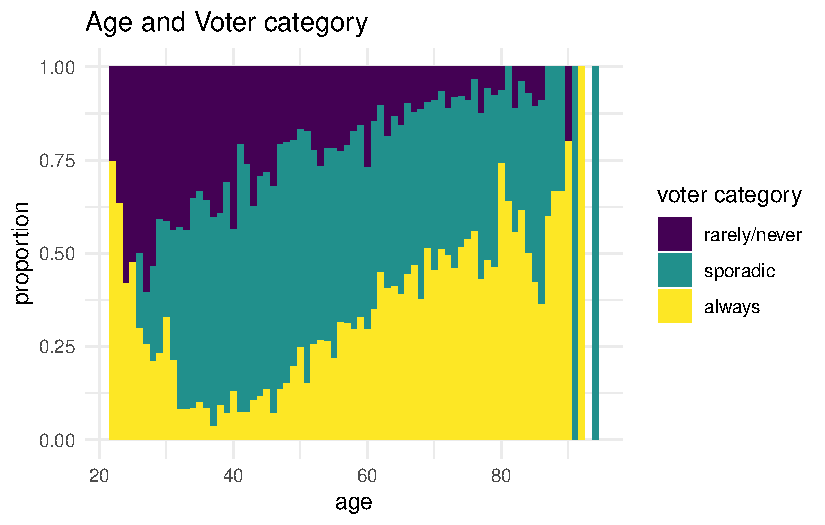
\includegraphics[keepaspectratio]{Lab_MultinomialRegression_files/figure-pdf/unnamed-chunk-6-1.pdf}}

\begin{Shaded}
\begin{Highlighting}[]
\CommentTok{\# Plot 2}
\NormalTok{voter\_data}\SpecialCharTok{$}\NormalTok{income\_cat }\OtherTok{\textless{}{-}} \FunctionTok{factor}\NormalTok{(voter\_data}\SpecialCharTok{$}\NormalTok{income\_cat, }
                \AttributeTok{levels =} \FunctionTok{c}\NormalTok{(}\StringTok{"Less than $40k"}\NormalTok{, }\StringTok{"$40{-}75k"}\NormalTok{, }\StringTok{"$75{-}125k"}\NormalTok{, }\StringTok{"$125k or more"}\NormalTok{), }
                \AttributeTok{ordered =} \ConstantTok{TRUE}\NormalTok{)}

\NormalTok{plot2 }\OtherTok{\textless{}{-}} \FunctionTok{ggplot}\NormalTok{(voter\_data, }\FunctionTok{aes}\NormalTok{(}\AttributeTok{x=}\NormalTok{ income\_cat, }\AttributeTok{fill =}\NormalTok{ voter\_category)) }\SpecialCharTok{+}
  \FunctionTok{geom\_bar}\NormalTok{(}\AttributeTok{position =} \StringTok{"fill"}\NormalTok{) }\SpecialCharTok{+}
  \FunctionTok{labs}\NormalTok{(}\AttributeTok{title =} \StringTok{"Income and Voter category"}\NormalTok{,}
       \AttributeTok{x =} \StringTok{"income category"}\NormalTok{,}
       \AttributeTok{y =} \StringTok{"proportion"}\NormalTok{,}
       \AttributeTok{fill =} \StringTok{"voter category"}\NormalTok{) }\SpecialCharTok{+}
  \FunctionTok{theme\_minimal}\NormalTok{()}

\NormalTok{plot2}
\end{Highlighting}
\end{Shaded}

\pandocbounded{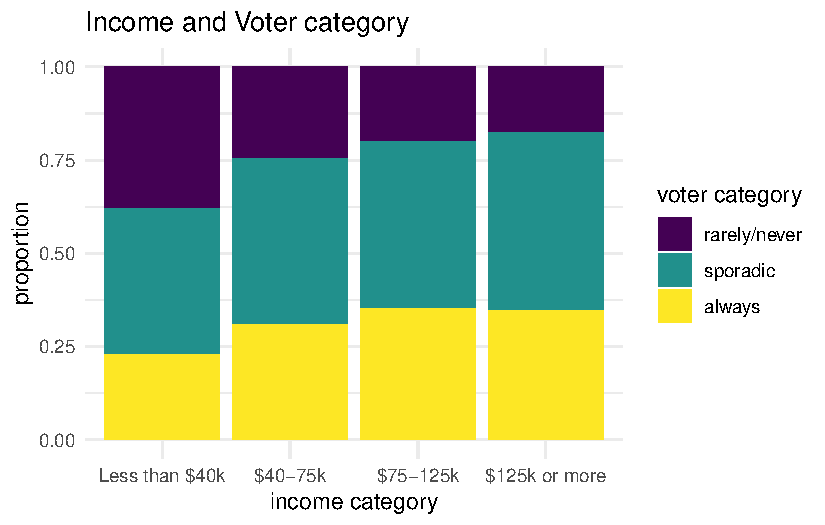
\includegraphics[keepaspectratio]{Lab_MultinomialRegression_files/figure-pdf/unnamed-chunk-7-1.pdf}}

\begin{Shaded}
\begin{Highlighting}[]
\CommentTok{\# Combine with patchwork}
\NormalTok{plot1 }\SpecialCharTok{+}\NormalTok{ plot2}
\end{Highlighting}
\end{Shaded}

\pandocbounded{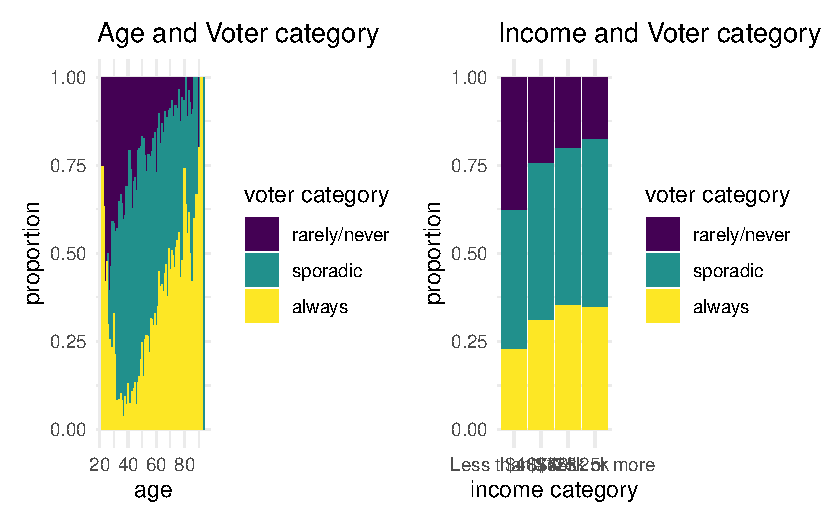
\includegraphics[keepaspectratio]{Lab_MultinomialRegression_files/figure-pdf/unnamed-chunk-8-1.pdf}}

\begin{quote}
Enter your interpretation here: (1) People generally tend to vote more
often as they get older, but only after age 30. The voting tendency
seems to decrease over time for young adults. (2) Regarding income
category, the richer people are, the more often they vote. The trend is
salient between lower income categories.
\end{quote}

\begin{center}\rule{0.5\linewidth}{0.5pt}\end{center}

\section{Part 3: Model Building}\label{part-3-model-building}

\subsubsection*{Question 3.1}\label{question-3.1}
\addcontentsline{toc}{subsubsection}{Question 3.1}

Fit a multinomial logistic regression model using mean-centered age,
race, gender, income, and education to predict \texttt{voter\_category}.
Save this as \texttt{model\_demo}.

You don't need to display the output here --- we'll examine it in Part
4. If you want to peek at it, feel free to run
\texttt{summary(model\_demo)} in your console. There's no real harm in
displaying it via the code chunk, except that it'll make your rendered
page quite messy. \texttt{kable()} is better for clean tables.

\begin{tcolorbox}[enhanced jigsaw, toprule=.15mm, opacitybacktitle=0.6, coltitle=black, opacityback=0, bottomrule=.15mm, left=2mm, colframe=quarto-callout-tip-color-frame, leftrule=.75mm, toptitle=1mm, colbacktitle=quarto-callout-tip-color!10!white, rightrule=.15mm, colback=white, title=\textcolor{quarto-callout-tip-color}{\faLightbulb}\hspace{0.5em}{Hint}, arc=.35mm, bottomtitle=1mm, titlerule=0mm, breakable]

\texttt{multinom(voter\_category\ \textasciitilde{}\ age\_centered\ +\ race\ +\ gender\ +\ income\_cat\ +\ educ,\ data\ =\ voter\_data,\ trace\ =\ FALSE)}
--- the \texttt{trace\ =\ FALSE} suppresses the iteration output.

To keep the rendered document clean, add
\texttt{\#\textbar{}\ results:\ hide} to the chunk header --- this runs
the code but hides the output. You can always check the output
interactively by running the chunk in the console.

\end{tcolorbox}

\begin{Shaded}
\begin{Highlighting}[]
\CommentTok{\# Enter your code}
\NormalTok{model\_demo }\OtherTok{\textless{}{-}} \FunctionTok{multinom}\NormalTok{(voter\_category }\SpecialCharTok{\textasciitilde{}}\NormalTok{ ppage\_mc }\SpecialCharTok{+}\NormalTok{ race }\SpecialCharTok{+}\NormalTok{ gender }\SpecialCharTok{+}\NormalTok{ income\_cat }\SpecialCharTok{+}\NormalTok{ educ, }\AttributeTok{data =}\NormalTok{ voter\_data, }\AttributeTok{trace =} \ConstantTok{FALSE}\NormalTok{)}
\end{Highlighting}
\end{Shaded}

\subsubsection*{Question 3.2}\label{question-3.2}
\addcontentsline{toc}{subsubsection}{Question 3.2}

Should party identification (\texttt{pol\_ident}) be added to the model?
Fit a second model that adds \texttt{pol\_ident} to the predictors. Use
\texttt{anova()} to compare the two models. Report the test statistic
and your conclusion.

\begin{Shaded}
\begin{Highlighting}[]
\CommentTok{\# Enter your code}
\NormalTok{model\_demo\_2 }\OtherTok{\textless{}{-}} \FunctionTok{multinom}\NormalTok{(voter\_category }\SpecialCharTok{\textasciitilde{}}\NormalTok{ ppage\_mc }\SpecialCharTok{+}\NormalTok{ race }\SpecialCharTok{+}\NormalTok{ gender }\SpecialCharTok{+}\NormalTok{ income\_cat }\SpecialCharTok{+}\NormalTok{ educ }\SpecialCharTok{+}\NormalTok{ pol\_ident, }\AttributeTok{data =}\NormalTok{ voter\_data, }\AttributeTok{trace =} \ConstantTok{FALSE}\NormalTok{)}

\FunctionTok{anova}\NormalTok{(model\_demo, model\_demo\_2)}
\end{Highlighting}
\end{Shaded}

\begin{verbatim}
Likelihood ratio tests of Multinomial Models

Response: voter_category
                                                     Model Resid. df Resid. Dev
1             ppage_mc + race + gender + income_cat + educ     11650   11386.63
2 ppage_mc + race + gender + income_cat + educ + pol_ident     11644   11232.78
    Test    Df LR stat. Pr(Chi)
1                              
2 1 vs 2     6  153.844       0
\end{verbatim}

\begin{Shaded}
\begin{Highlighting}[]
\NormalTok{final\_model }\OtherTok{\textless{}{-}}\NormalTok{ model\_demo\_2}
\end{Highlighting}
\end{Shaded}

\begin{quote}
Enter your answer: The likelihood ratio test shows that adding
pol\_ident variable as a predictor significantly improves the model
(\(\chi^2(6) = 153.84, p < .001\)).
\end{quote}

\textbf{Use the model you select for the remainder of the assignment.}
For clarity, call your chosen model \texttt{final\_model}.

\begin{center}\rule{0.5\linewidth}{0.5pt}\end{center}

\section{Part 4: Interpreting the
Model}\label{part-4-interpreting-the-model}

\subsubsection*{Question 4.1: Overall
significance}\label{question-4.1-overall-significance}
\addcontentsline{toc}{subsubsection}{Question 4.1: Overall significance}

Use a likelihood ratio test (\texttt{car::Anova()} with
\texttt{type\ =\ "III"}) to report the overall significance of each
predictor in \texttt{final\_model}.

\begin{Shaded}
\begin{Highlighting}[]
\CommentTok{\# Enter your code}
\NormalTok{car}\SpecialCharTok{::}\FunctionTok{Anova}\NormalTok{(final\_model, }\AttributeTok{type =} \StringTok{"III"}\NormalTok{)}
\end{Highlighting}
\end{Shaded}

\begin{verbatim}
Analysis of Deviance Table (Type III tests)

Response: voter_category
           LR Chisq Df Pr(>Chisq)    
ppage_mc     638.30  2  < 2.2e-16 ***
race          52.65  6  1.379e-09 ***
gender         6.03  2     0.0491 *  
income_cat    67.72  6  1.198e-12 ***
educ         154.14  4  < 2.2e-16 ***
pol_ident    153.84  6  < 2.2e-16 ***
---
Signif. codes:  0 '***' 0.001 '**' 0.01 '*' 0.05 '.' 0.1 ' ' 1
\end{verbatim}

\subsubsection*{Question 4.2: Raw
coefficients}\label{question-4.2-raw-coefficients}
\addcontentsline{toc}{subsubsection}{Question 4.2: Raw coefficients}

Display the model output using
\texttt{tidy(final\_model)\ \%\textgreater{}\%\ kable(digits\ =\ 3)}.

Pick \textbf{one} comparison (e.g., ``sporadic vs.~rarely/never'') and
do the following:

\begin{enumerate}
\def\labelenumi{\alph{enumi})}
\tightlist
\item
  Write out the model equation for that comparison.
\item
  Interpret the coefficient for mean-centered age: what happens to the
  \textbf{odds} of being in that category (vs.~the baseline) for each
  additional year of age? Report the odds ratio \texttt{exp(β)}.
\end{enumerate}

\begin{tcolorbox}[enhanced jigsaw, toprule=.15mm, opacitybacktitle=0.6, coltitle=black, opacityback=0, bottomrule=.15mm, left=2mm, colframe=quarto-callout-tip-color-frame, leftrule=.75mm, toptitle=1mm, colbacktitle=quarto-callout-tip-color!10!white, rightrule=.15mm, colback=white, title=\textcolor{quarto-callout-tip-color}{\faLightbulb}\hspace{0.5em}{Hint: Reading the tidy() output}, arc=.35mm, bottomtitle=1mm, titlerule=0mm, breakable]

When you run \texttt{tidy(final\_model)}, you'll see a table with
columns like \texttt{y.level}, \texttt{term}, \texttt{estimate}, etc.
The table has \textbf{two blocks of rows} --- one block where
\texttt{y.level} is \texttt{sporadic}, and another where
\texttt{y.level} is \texttt{always}. Each block is a separate logistic
regression equation:

\begin{itemize}
\tightlist
\item
  The \texttt{sporadic} rows are the equation for: log-odds of sporadic
  \textbf{vs.~rarely/never}
\item
  The \texttt{always} rows are the equation for: log-odds of always
  \textbf{vs.~rarely/never}
\end{itemize}

Pick one of those two blocks. The \texttt{(Intercept)} row is
\(\beta_0\) and the \texttt{age\_centered} row is \(\beta_1\) for that
equation.

\end{tcolorbox}

\begin{Shaded}
\begin{Highlighting}[]
\CommentTok{\# Enter your code}
\FunctionTok{tidy}\NormalTok{(final\_model) }\SpecialCharTok{\%\textgreater{}\%} \FunctionTok{kable}\NormalTok{(}\AttributeTok{digits =} \DecValTok{3}\NormalTok{)}
\end{Highlighting}
\end{Shaded}

\begin{longtable}[]{@{}
  >{\raggedright\arraybackslash}p{(\linewidth - 10\tabcolsep) * \real{0.1286}}
  >{\raggedright\arraybackslash}p{(\linewidth - 10\tabcolsep) * \real{0.3429}}
  >{\raggedleft\arraybackslash}p{(\linewidth - 10\tabcolsep) * \real{0.1286}}
  >{\raggedleft\arraybackslash}p{(\linewidth - 10\tabcolsep) * \real{0.1429}}
  >{\raggedleft\arraybackslash}p{(\linewidth - 10\tabcolsep) * \real{0.1429}}
  >{\raggedleft\arraybackslash}p{(\linewidth - 10\tabcolsep) * \real{0.1143}}@{}}
\toprule\noalign{}
\begin{minipage}[b]{\linewidth}\raggedright
y.level
\end{minipage} & \begin{minipage}[b]{\linewidth}\raggedright
term
\end{minipage} & \begin{minipage}[b]{\linewidth}\raggedleft
estimate
\end{minipage} & \begin{minipage}[b]{\linewidth}\raggedleft
std.error
\end{minipage} & \begin{minipage}[b]{\linewidth}\raggedleft
statistic
\end{minipage} & \begin{minipage}[b]{\linewidth}\raggedleft
p.value
\end{minipage} \\
\midrule\noalign{}
\endhead
\bottomrule\noalign{}
\endlastfoot
sporadic & (Intercept) & 1.569 & 0.119 & 13.153 & 0.000 \\
sporadic & ppage\_mc & 0.046 & 0.002 & 19.654 & 0.000 \\
sporadic & raceHispanic & 0.040 & 0.128 & 0.314 & 0.753 \\
sporadic & raceOther/Mixed & -0.332 & 0.159 & -2.090 & 0.037 \\
sporadic & raceWhite & -0.078 & 0.108 & -0.719 & 0.472 \\
sporadic & genderMale & -0.090 & 0.072 & -1.248 & 0.212 \\
sporadic & income\_cat.L & 0.414 & 0.081 & 5.101 & 0.000 \\
sporadic & income\_cat.Q & -0.263 & 0.072 & -3.650 & 0.000 \\
sporadic & income\_cat.C & 0.074 & 0.071 & 1.033 & 0.302 \\
sporadic & educHigh school or less & -0.853 & 0.097 & -8.761 & 0.000 \\
sporadic & educSome college & -0.293 & 0.095 & -3.076 & 0.002 \\
sporadic & pol\_identIndep & -0.392 & 0.098 & -4.017 & 0.000 \\
sporadic & pol\_identOther & -0.940 & 0.106 & -8.853 & 0.000 \\
sporadic & pol\_identRep & -0.084 & 0.103 & -0.815 & 0.415 \\
always & (Intercept) & 1.366 & 0.128 & 10.627 & 0.000 \\
always & ppage\_mc & 0.058 & 0.003 & 22.688 & 0.000 \\
always & raceHispanic & -0.341 & 0.150 & -2.277 & 0.023 \\
always & raceOther/Mixed & -0.600 & 0.185 & -3.239 & 0.001 \\
always & raceWhite & 0.127 & 0.119 & 1.071 & 0.284 \\
always & genderMale & -0.192 & 0.080 & -2.413 & 0.016 \\
always & income\_cat.L & 0.483 & 0.090 & 5.344 & 0.000 \\
always & income\_cat.Q & -0.414 & 0.080 & -5.196 & 0.000 \\
always & income\_cat.C & 0.037 & 0.078 & 0.481 & 0.630 \\
always & educHigh school or less & -1.267 & 0.109 & -11.644 & 0.000 \\
always & educSome college & -0.330 & 0.102 & -3.225 & 0.001 \\
always & pol\_identIndep & -0.562 & 0.107 & -5.259 & 0.000 \\
always & pol\_identOther & -1.401 & 0.131 & -10.678 & 0.000 \\
always & pol\_identRep & -0.162 & 0.110 & -1.469 & 0.142 \\
\end{longtable}

\begin{Shaded}
\begin{Highlighting}[]
\FunctionTok{exp}\NormalTok{(}\FloatTok{0.058}\NormalTok{)}
\end{Highlighting}
\end{Shaded}

\begin{verbatim}
[1] 1.059715
\end{verbatim}

\begin{Shaded}
\begin{Highlighting}[]
\NormalTok{coef\_age }\OtherTok{\textless{}{-}} \FunctionTok{tidy}\NormalTok{(final\_model) }\SpecialCharTok{\%\textgreater{}\%} 
\NormalTok{  dplyr}\SpecialCharTok{::}\FunctionTok{filter}\NormalTok{(term }\SpecialCharTok{==} \StringTok{"ppage\_mc"}\NormalTok{, y.level }\SpecialCharTok{==} \StringTok{"always"}\NormalTok{)}
\NormalTok{beta }\OtherTok{\textless{}{-}}\NormalTok{ coef\_age}\SpecialCharTok{$}\NormalTok{estimate}
\NormalTok{se }\OtherTok{\textless{}{-}}\NormalTok{ coef\_age}\SpecialCharTok{$}\NormalTok{std.error}
\NormalTok{lower }\OtherTok{\textless{}{-}} \FunctionTok{exp}\NormalTok{(beta }\SpecialCharTok{{-}} \FloatTok{1.96} \SpecialCharTok{*}\NormalTok{ se)}
\NormalTok{upper }\OtherTok{\textless{}{-}} \FunctionTok{exp}\NormalTok{(beta }\SpecialCharTok{+} \FloatTok{1.96} \SpecialCharTok{*}\NormalTok{ se)}
\FunctionTok{c}\NormalTok{(lower, upper)}
\end{Highlighting}
\end{Shaded}

\begin{verbatim}
[1] 1.054618 1.065278
\end{verbatim}

\begin{Shaded}
\begin{Highlighting}[]
\FunctionTok{exp}\NormalTok{(beta)}
\end{Highlighting}
\end{Shaded}

\begin{verbatim}
[1] 1.059935
\end{verbatim}

\begin{quote}
Enter your equation and interpretation here: (rarely/never vs.~always)
voter\_category = 1.366 + 0.058 * ppage\_mc + (-0.341)*raceHispanic +
\ldots{} + (-0.162)*pol\_identRep

With each additional year of age, the odds of being in `always' category
(rather than `rarely/never' category) increases about 6\%.
\end{quote}

\subsubsection*{Question 4.3: Changing the
baseline}\label{question-4.3-changing-the-baseline}
\addcontentsline{toc}{subsubsection}{Question 4.3: Changing the
baseline}

Refit the model with a \textbf{different} baseline category for
\texttt{voter\_category} (e.g., ``always'' instead of ``rarely/never'').
Then predict the probabilities for a specific observation using both
models.

Do the coefficients change? Do the predicted probabilities change?
Explain in 1--2 sentences why this happens.

\begin{tcolorbox}[enhanced jigsaw, toprule=.15mm, opacitybacktitle=0.6, coltitle=black, opacityback=0, bottomrule=.15mm, left=2mm, colframe=quarto-callout-tip-color-frame, leftrule=.75mm, toptitle=1mm, colbacktitle=quarto-callout-tip-color!10!white, rightrule=.15mm, colback=white, title=\textcolor{quarto-callout-tip-color}{\faLightbulb}\hspace{0.5em}{Hint}, arc=.35mm, bottomtitle=1mm, titlerule=0mm, breakable]

Use \texttt{relevel(voter\_category,\ ref\ =\ "always")} before
refitting. Use
\texttt{predict(model,\ newdata\ =\ ...,\ type\ =\ "probs")} to get
predicted probabilities. You can use \texttt{head(voter\_data,\ 1)} as
your newdata for a quick check.

\end{tcolorbox}

\begin{Shaded}
\begin{Highlighting}[]
\CommentTok{\# Enter your code}
\NormalTok{voter\_data}\SpecialCharTok{$}\NormalTok{voter\_category }\OtherTok{\textless{}{-}} \FunctionTok{relevel}\NormalTok{(}\FunctionTok{factor}\NormalTok{(voter\_data}\SpecialCharTok{$}\NormalTok{voter\_category, }\AttributeTok{ordered =} \ConstantTok{FALSE}\NormalTok{), }\AttributeTok{ref =} \StringTok{"always"}\NormalTok{)}

\NormalTok{model\_refit }\OtherTok{\textless{}{-}} \FunctionTok{multinom}\NormalTok{(voter\_category }\SpecialCharTok{\textasciitilde{}}\NormalTok{ ppage\_mc }\SpecialCharTok{+}\NormalTok{ race }\SpecialCharTok{+}\NormalTok{ gender }\SpecialCharTok{+}\NormalTok{ income\_cat }\SpecialCharTok{+}\NormalTok{ educ }\SpecialCharTok{+}\NormalTok{ pol\_ident, }\AttributeTok{data =}\NormalTok{ voter\_data, }\AttributeTok{trace =} \ConstantTok{FALSE}\NormalTok{)}

\FunctionTok{tidy}\NormalTok{(model\_refit) }\SpecialCharTok{\%\textgreater{}\%} \FunctionTok{kable}\NormalTok{(}\AttributeTok{digits =} \DecValTok{3}\NormalTok{)}
\end{Highlighting}
\end{Shaded}

\begin{longtable}[]{@{}
  >{\raggedright\arraybackslash}p{(\linewidth - 10\tabcolsep) * \real{0.1757}}
  >{\raggedright\arraybackslash}p{(\linewidth - 10\tabcolsep) * \real{0.3243}}
  >{\raggedleft\arraybackslash}p{(\linewidth - 10\tabcolsep) * \real{0.1216}}
  >{\raggedleft\arraybackslash}p{(\linewidth - 10\tabcolsep) * \real{0.1351}}
  >{\raggedleft\arraybackslash}p{(\linewidth - 10\tabcolsep) * \real{0.1351}}
  >{\raggedleft\arraybackslash}p{(\linewidth - 10\tabcolsep) * \real{0.1081}}@{}}
\toprule\noalign{}
\begin{minipage}[b]{\linewidth}\raggedright
y.level
\end{minipage} & \begin{minipage}[b]{\linewidth}\raggedright
term
\end{minipage} & \begin{minipage}[b]{\linewidth}\raggedleft
estimate
\end{minipage} & \begin{minipage}[b]{\linewidth}\raggedleft
std.error
\end{minipage} & \begin{minipage}[b]{\linewidth}\raggedleft
statistic
\end{minipage} & \begin{minipage}[b]{\linewidth}\raggedleft
p.value
\end{minipage} \\
\midrule\noalign{}
\endhead
\bottomrule\noalign{}
\endlastfoot
rarely/never & (Intercept) & -1.366 & 0.128 & -10.628 & 0.000 \\
rarely/never & ppage\_mc & -0.058 & 0.003 & -22.688 & 0.000 \\
rarely/never & raceHispanic & 0.341 & 0.150 & 2.277 & 0.023 \\
rarely/never & raceOther/Mixed & 0.600 & 0.185 & 3.239 & 0.001 \\
rarely/never & raceWhite & -0.127 & 0.119 & -1.071 & 0.284 \\
rarely/never & genderMale & 0.192 & 0.080 & 2.413 & 0.016 \\
rarely/never & income\_cat.L & -0.483 & 0.090 & -5.344 & 0.000 \\
rarely/never & income\_cat.Q & 0.414 & 0.080 & 5.196 & 0.000 \\
rarely/never & income\_cat.C & -0.037 & 0.078 & -0.481 & 0.630 \\
rarely/never & educHigh school or less & 1.267 & 0.109 & 11.644 &
0.000 \\
rarely/never & educSome college & 0.330 & 0.102 & 3.226 & 0.001 \\
rarely/never & pol\_identIndep & 0.562 & 0.107 & 5.259 & 0.000 \\
rarely/never & pol\_identOther & 1.401 & 0.131 & 10.678 & 0.000 \\
rarely/never & pol\_identRep & 0.162 & 0.110 & 1.469 & 0.142 \\
sporadic & (Intercept) & 0.204 & 0.094 & 2.165 & 0.030 \\
sporadic & ppage\_mc & -0.013 & 0.002 & -6.375 & 0.000 \\
sporadic & raceHispanic & 0.381 & 0.122 & 3.118 & 0.002 \\
sporadic & raceOther/Mixed & 0.268 & 0.156 & 1.717 & 0.086 \\
sporadic & raceWhite & -0.205 & 0.093 & -2.210 & 0.027 \\
sporadic & genderMale & 0.102 & 0.063 & 1.615 & 0.106 \\
sporadic & income\_cat.L & -0.069 & 0.073 & -0.944 & 0.345 \\
sporadic & income\_cat.Q & 0.151 & 0.063 & 2.388 & 0.017 \\
sporadic & income\_cat.C & 0.036 & 0.061 & 0.595 & 0.552 \\
sporadic & educHigh school or less & 0.414 & 0.087 & 4.758 & 0.000 \\
sporadic & educSome college & 0.037 & 0.077 & 0.484 & 0.629 \\
sporadic & pol\_identIndep & 0.170 & 0.084 & 2.021 & 0.043 \\
sporadic & pol\_identOther & 0.461 & 0.121 & 3.801 & 0.000 \\
sporadic & pol\_identRep & 0.078 & 0.082 & 0.952 & 0.341 \\
\end{longtable}

\begin{Shaded}
\begin{Highlighting}[]
\FunctionTok{predict}\NormalTok{(model\_refit, }\AttributeTok{newdata =} \FunctionTok{head}\NormalTok{(voter\_data, }\DecValTok{1}\NormalTok{), }\AttributeTok{type =} \StringTok{"probs"}\NormalTok{)}
\end{Highlighting}
\end{Shaded}

\begin{verbatim}
      always rarely/never     sporadic 
  0.57788857   0.02811795   0.39399348 
\end{verbatim}

\begin{Shaded}
\begin{Highlighting}[]
\FunctionTok{predict}\NormalTok{(final\_model, }\AttributeTok{newdata =} \FunctionTok{head}\NormalTok{(voter\_data, }\DecValTok{1}\NormalTok{), }\AttributeTok{type =} \StringTok{"probs"}\NormalTok{)}
\end{Highlighting}
\end{Shaded}

\begin{verbatim}
rarely/never     sporadic       always 
  0.02811839   0.39399517   0.57788644 
\end{verbatim}

\begin{quote}
Enter your answer: The coefficients change as baseline changes because
they are calculated relative to the reference category. Whereas the
predicted probabilities remain the same as the model predictions for
each category don't change.
\end{quote}

\begin{center}\rule{0.5\linewidth}{0.5pt}\end{center}

\section{Part 5: Marginal Effects \&
Visualization}\label{part-5-marginal-effects-visualization}

\subsubsection*{Question 5.1: Predicted probabilities by
age}\label{question-5.1-predicted-probabilities-by-age}
\addcontentsline{toc}{subsubsection}{Question 5.1: Predicted
probabilities by age}

Plot the predicted probabilities of voter category as a function of age.
The code below will work once you replace \texttt{final\_model} with the
name of your model:

\begin{tcolorbox}[enhanced jigsaw, toprule=.15mm, opacitybacktitle=0.6, coltitle=black, opacityback=0, bottomrule=.15mm, left=2mm, colframe=quarto-callout-note-color-frame, leftrule=.75mm, toptitle=1mm, colbacktitle=quarto-callout-note-color!10!white, rightrule=.15mm, colback=white, title=\textcolor{quarto-callout-note-color}{\faInfo}\hspace{0.5em}{Note}, arc=.35mm, bottomtitle=1mm, titlerule=0mm, breakable]

This chunk is set to \texttt{eval:\ false} so the file renders before
you've built your model. Once \texttt{final\_model} exists in your
environment, delete the \texttt{\#\textbar{}\ eval:\ false} line so the
chunk runs when you render.

\end{tcolorbox}

\begin{Shaded}
\begin{Highlighting}[]
\FunctionTok{ggemmeans}\NormalTok{(final\_model, }\AttributeTok{terms =} \FunctionTok{c}\NormalTok{(}\StringTok{"ppage\_mc [n=25]"}\NormalTok{)) }\SpecialCharTok{\%\textgreater{}\%}
  \FunctionTok{ggplot}\NormalTok{(., }\FunctionTok{aes}\NormalTok{(}\AttributeTok{x =}\NormalTok{ x, }\AttributeTok{y =}\NormalTok{ predicted, }\AttributeTok{fill =}\NormalTok{ response.level)) }\SpecialCharTok{+}
  \FunctionTok{geom\_area}\NormalTok{() }\SpecialCharTok{+}
  \FunctionTok{geom\_rug}\NormalTok{(}\AttributeTok{sides =} \StringTok{"b"}\NormalTok{, }\AttributeTok{position =} \StringTok{"jitter"}\NormalTok{, }\AttributeTok{alpha =}\NormalTok{ .}\DecValTok{2}\NormalTok{) }\SpecialCharTok{+}
  \FunctionTok{labs}\NormalTok{(}\AttributeTok{x =} \StringTok{"}\SpecialCharTok{\textbackslash{}n}\StringTok{Age"}\NormalTok{, }\AttributeTok{y =} \StringTok{"Predicted Probability}\SpecialCharTok{\textbackslash{}n}\StringTok{"}\NormalTok{,}
       \AttributeTok{title =} \StringTok{"Predicted Probabilities of Voting Frequency by Age"}\NormalTok{) }\SpecialCharTok{+}
  \FunctionTok{scale\_fill\_manual}\NormalTok{(}
    \AttributeTok{name =} \ConstantTok{NULL}\NormalTok{,}
    \AttributeTok{values =} \FunctionTok{c}\NormalTok{(}\StringTok{"always"} \OtherTok{=} \StringTok{"\#F6B533"}\NormalTok{, }\StringTok{"sporadic"} \OtherTok{=} \StringTok{"\#D07EA2"}\NormalTok{, }\StringTok{"rarely/never"} \OtherTok{=} \StringTok{"\#9854F7"}\NormalTok{),}
    \AttributeTok{labels =} \FunctionTok{c}\NormalTok{(}\StringTok{"RARELY OR NEVER VOTE    "}\NormalTok{, }\StringTok{"SOMETIMES VOTE    "}\NormalTok{, }\StringTok{"ALMOST ALWAYS VOTE    "}\NormalTok{),}
    \AttributeTok{breaks =} \FunctionTok{c}\NormalTok{(}\StringTok{"rarely/never"}\NormalTok{, }\StringTok{"sporadic"}\NormalTok{, }\StringTok{"always"}\NormalTok{)}
\NormalTok{  ) }\SpecialCharTok{+}
  \FunctionTok{theme\_minimal}\NormalTok{()}
\end{Highlighting}
\end{Shaded}

\pandocbounded{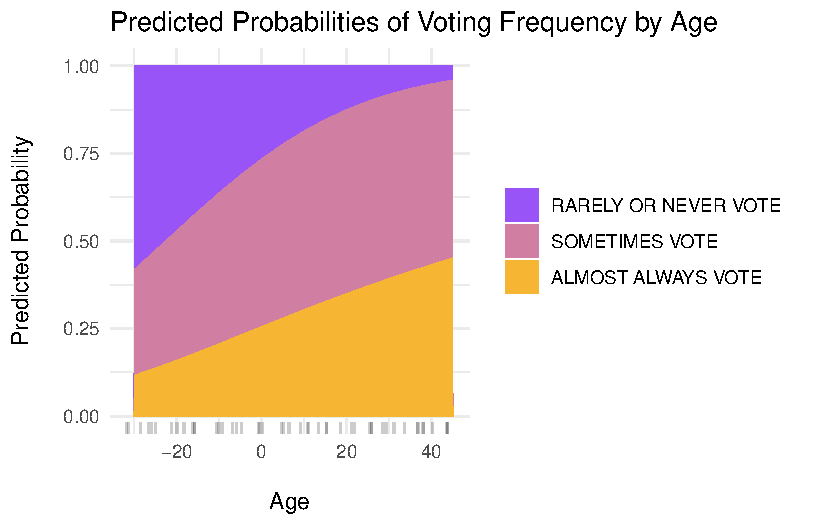
\includegraphics[keepaspectratio]{Lab_MultinomialRegression_files/figure-pdf/unnamed-chunk-14-1.pdf}}

\begin{Shaded}
\begin{Highlighting}[]
\CommentTok{\#ppage\_mc [all] didn\textquotesingle{}t work; the error message said the rows of my requested reference grid (i.e., 14208) exceeded the limit of 10000.}
\end{Highlighting}
\end{Shaded}

Describe the pattern you see in 1--2 sentences.

\begin{quote}
Enter your interpretation here: Voting behavior increases as people get
older. The probabilities of `sometimes voting' is highest in young
adults but declines for older population.
\end{quote}

\subsubsection*{Question 5.2: Predicted probabilities by
education}\label{question-5.2-predicted-probabilities-by-education}
\addcontentsline{toc}{subsubsection}{Question 5.2: Predicted
probabilities by education}

Create a similar plot showing predicted probabilities of voter category
as a function of \textbf{education level}.

\begin{tcolorbox}[enhanced jigsaw, toprule=.15mm, opacitybacktitle=0.6, coltitle=black, opacityback=0, bottomrule=.15mm, left=2mm, colframe=quarto-callout-tip-color-frame, leftrule=.75mm, toptitle=1mm, colbacktitle=quarto-callout-tip-color!10!white, rightrule=.15mm, colback=white, title=\textcolor{quarto-callout-tip-color}{\faLightbulb}\hspace{0.5em}{Hint}, arc=.35mm, bottomtitle=1mm, titlerule=0mm, breakable]

Replace \texttt{"ppage\ {[}all{]}"} with \texttt{"educ"} in the
\texttt{ggemmeans()} call. Since education is categorical, you may want
to use \texttt{geom\_col(position\ =\ "dodge")} or
\texttt{geom\_col(position\ =\ "fill")} instead of
\texttt{geom\_area()}.

\end{tcolorbox}

\begin{Shaded}
\begin{Highlighting}[]
\CommentTok{\# Enter your code}
\FunctionTok{ggemmeans}\NormalTok{(final\_model, }\AttributeTok{terms =} \FunctionTok{c}\NormalTok{(}\StringTok{"educ"}\NormalTok{)) }\SpecialCharTok{\%\textgreater{}\%}
  \FunctionTok{ggplot}\NormalTok{(., }\FunctionTok{aes}\NormalTok{(}\AttributeTok{x =}\NormalTok{ x, }\AttributeTok{y =}\NormalTok{ predicted, }\AttributeTok{fill =}\NormalTok{ response.level)) }\SpecialCharTok{+}
  \FunctionTok{geom\_col}\NormalTok{(}\AttributeTok{position =} \StringTok{"fill"}\NormalTok{) }\SpecialCharTok{+}
  \FunctionTok{geom\_rug}\NormalTok{(}\AttributeTok{sides =} \StringTok{"b"}\NormalTok{, }\AttributeTok{position =} \StringTok{"jitter"}\NormalTok{, }\AttributeTok{alpha =}\NormalTok{ .}\DecValTok{2}\NormalTok{) }\SpecialCharTok{+}
  \FunctionTok{labs}\NormalTok{(}\AttributeTok{x =} \StringTok{"}\SpecialCharTok{\textbackslash{}n}\StringTok{Age"}\NormalTok{, }\AttributeTok{y =} \StringTok{"Predicted Probability}\SpecialCharTok{\textbackslash{}n}\StringTok{"}\NormalTok{,}
       \AttributeTok{title =} \StringTok{"Predicted Probabilities of Voting Frequency by Education level"}\NormalTok{) }\SpecialCharTok{+}
  \FunctionTok{scale\_fill\_manual}\NormalTok{(}
    \AttributeTok{name =} \ConstantTok{NULL}\NormalTok{,}
    \AttributeTok{values =} \FunctionTok{c}\NormalTok{(}\StringTok{"always"} \OtherTok{=} \StringTok{"\#F6B533"}\NormalTok{, }\StringTok{"sporadic"} \OtherTok{=} \StringTok{"\#D07EA2"}\NormalTok{, }\StringTok{"rarely/never"} \OtherTok{=} \StringTok{"\#9854F7"}\NormalTok{),}
    \AttributeTok{labels =} \FunctionTok{c}\NormalTok{(}\StringTok{"RARELY OR NEVER VOTE    "}\NormalTok{, }\StringTok{"SOMETIMES VOTE    "}\NormalTok{, }\StringTok{"ALMOST ALWAYS VOTE    "}\NormalTok{),}
    \AttributeTok{breaks =} \FunctionTok{c}\NormalTok{(}\StringTok{"rarely/never"}\NormalTok{, }\StringTok{"sporadic"}\NormalTok{, }\StringTok{"always"}\NormalTok{)}
\NormalTok{  ) }\SpecialCharTok{+}
  \FunctionTok{theme\_minimal}\NormalTok{()}
\end{Highlighting}
\end{Shaded}

\pandocbounded{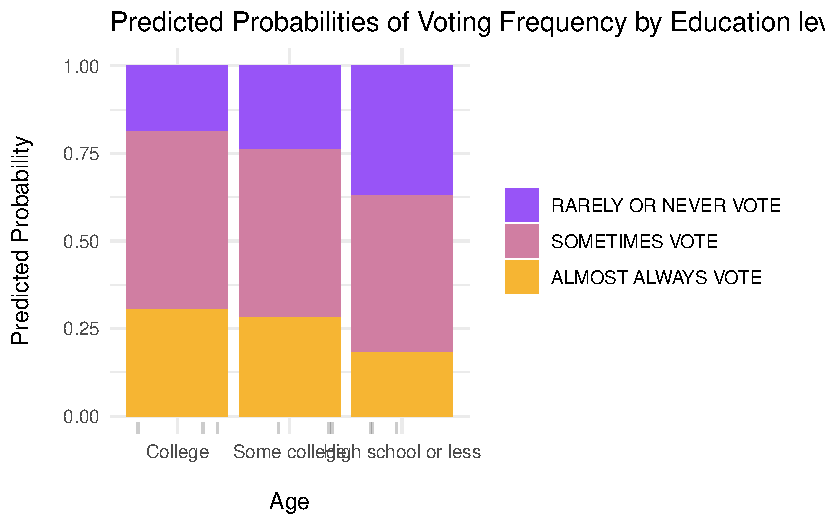
\includegraphics[keepaspectratio]{Lab_MultinomialRegression_files/figure-pdf/unnamed-chunk-15-1.pdf}}

\begin{quote}
Enter your interpretation here: Individuals with higher education level
tend to vote more often compared to individuals with lower education
level. The probability of `rarely or never voting' is the highest in
`high school or less' group and the lowest in `college' group. The
probability of `almost always voting' showed the opposite trend.
\end{quote}

\begin{center}\rule{0.5\linewidth}{0.5pt}\end{center}

\section{Part 6: Pairwise
Comparisons}\label{part-6-pairwise-comparisons}

\subsubsection*{Question 6.1: Political group
differences}\label{question-6.1-political-group-differences}
\addcontentsline{toc}{subsubsection}{Question 6.1: Political group
differences}

Run the following code (replacing \texttt{final\_model} with your model
name) and interpret the output. The code computes estimated marginal
means for each political group within each voter category, then tests
pairwise differences on the log-odds scale.

\begin{tcolorbox}[enhanced jigsaw, toprule=.15mm, opacitybacktitle=0.6, coltitle=black, opacityback=0, bottomrule=.15mm, left=2mm, colframe=quarto-callout-note-color-frame, leftrule=.75mm, toptitle=1mm, colbacktitle=quarto-callout-note-color!10!white, rightrule=.15mm, colback=white, title=\textcolor{quarto-callout-note-color}{\faInfo}\hspace{0.5em}{Note}, arc=.35mm, bottomtitle=1mm, titlerule=0mm, breakable]

Same as Q5.1 --- this chunk is set to \texttt{eval:\ false}. Delete that
line once \texttt{final\_model} exists.

\end{tcolorbox}

\begin{Shaded}
\begin{Highlighting}[]
\CommentTok{\# Estimated marginal means: political group by voter category}
\NormalTok{multi\_an\_pol }\OtherTok{\textless{}{-}} \FunctionTok{emmeans}\NormalTok{(final\_model, }\SpecialCharTok{\textasciitilde{}}\NormalTok{ pol\_ident }\SpecialCharTok{|}\NormalTok{ voter\_category)}

\CommentTok{\# Contrasts on the log scale (log{-}odds differences between voter categories, within each political group)}
\NormalTok{coefs\_pol }\OtherTok{\textless{}{-}} \FunctionTok{contrast}\NormalTok{(}\FunctionTok{regrid}\NormalTok{(multi\_an\_pol, }\StringTok{"log"}\NormalTok{), }\StringTok{"trt.vs.ctrl1"}\NormalTok{, }\AttributeTok{by =} \StringTok{"pol\_ident"}\NormalTok{)}

\CommentTok{\# Display results, organized by contrast}
\FunctionTok{update}\NormalTok{(coefs\_pol, }\AttributeTok{by =} \StringTok{"contrast"}\NormalTok{) }\SpecialCharTok{\%\textgreater{}\%}
  \FunctionTok{kable}\NormalTok{(}\AttributeTok{format =} \StringTok{"markdown"}\NormalTok{, }\AttributeTok{digits =} \DecValTok{3}\NormalTok{)}
\end{Highlighting}
\end{Shaded}

\begin{longtable}[]{@{}
  >{\raggedright\arraybackslash}p{(\linewidth - 12\tabcolsep) * \real{0.3714}}
  >{\raggedright\arraybackslash}p{(\linewidth - 12\tabcolsep) * \real{0.1429}}
  >{\raggedleft\arraybackslash}p{(\linewidth - 12\tabcolsep) * \real{0.1286}}
  >{\raggedleft\arraybackslash}p{(\linewidth - 12\tabcolsep) * \real{0.0857}}
  >{\raggedleft\arraybackslash}p{(\linewidth - 12\tabcolsep) * \real{0.0429}}
  >{\raggedleft\arraybackslash}p{(\linewidth - 12\tabcolsep) * \real{0.1143}}
  >{\raggedleft\arraybackslash}p{(\linewidth - 12\tabcolsep) * \real{0.1143}}@{}}
\toprule\noalign{}
\begin{minipage}[b]{\linewidth}\raggedright
contrast
\end{minipage} & \begin{minipage}[b]{\linewidth}\raggedright
pol\_ident
\end{minipage} & \begin{minipage}[b]{\linewidth}\raggedleft
estimate
\end{minipage} & \begin{minipage}[b]{\linewidth}\raggedleft
SE
\end{minipage} & \begin{minipage}[b]{\linewidth}\raggedleft
df
\end{minipage} & \begin{minipage}[b]{\linewidth}\raggedleft
t.ratio
\end{minipage} & \begin{minipage}[b]{\linewidth}\raggedleft
p.value
\end{minipage} \\
\midrule\noalign{}
\endhead
\bottomrule\noalign{}
\endlastfoot
sporadic - (rarely/never) & Dem & 0.961 & 0.070 & 28 & 13.722 & 0.000 \\
always - (rarely/never) & Dem & 0.480 & 0.074 & 28 & 6.498 & 0.000 \\
sporadic - (rarely/never) & Indep & 0.591 & 0.077 & 28 & 7.643 &
0.000 \\
always - (rarely/never) & Indep & -0.049 & 0.084 & 28 & -0.589 &
0.900 \\
sporadic - (rarely/never) & Other & 0.078 & 0.087 & 28 & 0.901 &
0.747 \\
always - (rarely/never) & Other & -0.835 & 0.110 & 28 & -7.577 &
0.000 \\
sporadic - (rarely/never) & Rep & 0.883 & 0.084 & 28 & 10.469 & 0.000 \\
always - (rarely/never) & Rep & 0.327 & 0.089 & 28 & 3.672 & 0.004 \\
\end{longtable}

\begin{Shaded}
\begin{Highlighting}[]
\CommentTok{\# Pairwise differences between political groups, within each contrast}
\FunctionTok{contrast}\NormalTok{(coefs\_pol, }\StringTok{"revpairwise"}\NormalTok{, }\AttributeTok{by =} \StringTok{"contrast"}\NormalTok{) }\SpecialCharTok{\%\textgreater{}\%}
  \FunctionTok{kable}\NormalTok{(}\AttributeTok{format =} \StringTok{"markdown"}\NormalTok{, }\AttributeTok{digits =} \DecValTok{3}\NormalTok{)}
\end{Highlighting}
\end{Shaded}

\begin{longtable}[]{@{}
  >{\raggedright\arraybackslash}p{(\linewidth - 12\tabcolsep) * \real{0.1892}}
  >{\raggedright\arraybackslash}p{(\linewidth - 12\tabcolsep) * \real{0.3514}}
  >{\raggedleft\arraybackslash}p{(\linewidth - 12\tabcolsep) * \real{0.1216}}
  >{\raggedleft\arraybackslash}p{(\linewidth - 12\tabcolsep) * \real{0.0811}}
  >{\raggedleft\arraybackslash}p{(\linewidth - 12\tabcolsep) * \real{0.0405}}
  >{\raggedleft\arraybackslash}p{(\linewidth - 12\tabcolsep) * \real{0.1081}}
  >{\raggedleft\arraybackslash}p{(\linewidth - 12\tabcolsep) * \real{0.1081}}@{}}
\toprule\noalign{}
\begin{minipage}[b]{\linewidth}\raggedright
contrast1
\end{minipage} & \begin{minipage}[b]{\linewidth}\raggedright
contrast
\end{minipage} & \begin{minipage}[b]{\linewidth}\raggedleft
estimate
\end{minipage} & \begin{minipage}[b]{\linewidth}\raggedleft
SE
\end{minipage} & \begin{minipage}[b]{\linewidth}\raggedleft
df
\end{minipage} & \begin{minipage}[b]{\linewidth}\raggedleft
t.ratio
\end{minipage} & \begin{minipage}[b]{\linewidth}\raggedleft
p.value
\end{minipage} \\
\midrule\noalign{}
\endhead
\bottomrule\noalign{}
\endlastfoot
Indep - Dem & sporadic - (rarely/never) & -0.370 & 0.094 & 28 & -3.933 &
0.003 \\
Other - Dem & sporadic - (rarely/never) & -0.883 & 0.103 & 28 & -8.578 &
0.000 \\
Other - Indep & sporadic - (rarely/never) & -0.513 & 0.107 & 28 & -4.807
& 0.000 \\
Rep - Dem & sporadic - (rarely/never) & -0.078 & 0.099 & 28 & -0.787 &
0.860 \\
Rep - Indep & sporadic - (rarely/never) & 0.292 & 0.099 & 28 & 2.965 &
0.029 \\
Rep - Other & sporadic - (rarely/never) & 0.805 & 0.109 & 28 & 7.404 &
0.000 \\
Indep - Dem & always - (rarely/never) & -0.529 & 0.101 & 28 & -5.254 &
0.000 \\
Other - Dem & always - (rarely/never) & -1.315 & 0.125 & 28 & -10.508 &
0.000 \\
Other - Indep & always - (rarely/never) & -0.786 & 0.129 & 28 & -6.072 &
0.000 \\
Rep - Dem & always - (rarely/never) & -0.153 & 0.104 & 28 & -1.470 &
0.468 \\
Rep - Indep & always - (rarely/never) & 0.376 & 0.104 & 28 & 3.605 &
0.006 \\
Rep - Other & always - (rarely/never) & 1.162 & 0.130 & 28 & 8.969 &
0.000 \\
\end{longtable}

\begin{quote}
Enter your interpretation here: Democratic and Republican voters are
significantly more likely to be sporadic or always voting rather than
rarely/never voting. Independent voters are more likely to be sporadic
voters and Others to be always voters, both compared to being
`rarely/never' voters. Democrats are significantly more likely to vote
sporaticaly or always (vs.~rarely/never) than other political identity
groups.
\end{quote}

\subsubsection*{Question 6.2: Education level
differences}\label{question-6.2-education-level-differences}
\addcontentsline{toc}{subsubsection}{Question 6.2: Education level
differences}

Adapt the code from 6.1 to examine differences across \textbf{education
levels} instead of political groups. Run it and interpret.

\begin{tcolorbox}[enhanced jigsaw, toprule=.15mm, opacitybacktitle=0.6, coltitle=black, opacityback=0, bottomrule=.15mm, left=2mm, colframe=quarto-callout-tip-color-frame, leftrule=.75mm, toptitle=1mm, colbacktitle=quarto-callout-tip-color!10!white, rightrule=.15mm, colback=white, title=\textcolor{quarto-callout-tip-color}{\faLightbulb}\hspace{0.5em}{Hint}, arc=.35mm, bottomtitle=1mm, titlerule=0mm, breakable]

Replace \texttt{pol\_ident} with \texttt{educ} in the \texttt{emmeans()}
and \texttt{contrast()} calls.

\end{tcolorbox}

\begin{Shaded}
\begin{Highlighting}[]
\CommentTok{\# Enter your code}
\CommentTok{\# Estimated marginal means: education level group by voter category}
\NormalTok{multi\_an\_educ }\OtherTok{\textless{}{-}} \FunctionTok{emmeans}\NormalTok{(final\_model, }\SpecialCharTok{\textasciitilde{}}\NormalTok{ educ }\SpecialCharTok{|}\NormalTok{ voter\_category)}

\CommentTok{\# Contrasts on the log scale (log{-}odds differences between voter categories, within each education level group)}
\NormalTok{coefs\_educ }\OtherTok{\textless{}{-}} \FunctionTok{contrast}\NormalTok{(}\FunctionTok{regrid}\NormalTok{(multi\_an\_educ, }\StringTok{"log"}\NormalTok{), }\StringTok{"trt.vs.ctrl1"}\NormalTok{, }\AttributeTok{by =} \StringTok{"educ"}\NormalTok{)}

\CommentTok{\# Display results, organized by contrast}
\FunctionTok{update}\NormalTok{(coefs\_educ, }\AttributeTok{by =} \StringTok{"contrast"}\NormalTok{) }\SpecialCharTok{\%\textgreater{}\%}
  \FunctionTok{kable}\NormalTok{(}\AttributeTok{format =} \StringTok{"markdown"}\NormalTok{, }\AttributeTok{digits =} \DecValTok{3}\NormalTok{)}
\end{Highlighting}
\end{Shaded}

\begin{longtable}[]{@{}
  >{\raggedright\arraybackslash}p{(\linewidth - 12\tabcolsep) * \real{0.3250}}
  >{\raggedright\arraybackslash}p{(\linewidth - 12\tabcolsep) * \real{0.2500}}
  >{\raggedleft\arraybackslash}p{(\linewidth - 12\tabcolsep) * \real{0.1125}}
  >{\raggedleft\arraybackslash}p{(\linewidth - 12\tabcolsep) * \real{0.0750}}
  >{\raggedleft\arraybackslash}p{(\linewidth - 12\tabcolsep) * \real{0.0375}}
  >{\raggedleft\arraybackslash}p{(\linewidth - 12\tabcolsep) * \real{0.1000}}
  >{\raggedleft\arraybackslash}p{(\linewidth - 12\tabcolsep) * \real{0.1000}}@{}}
\toprule\noalign{}
\begin{minipage}[b]{\linewidth}\raggedright
contrast
\end{minipage} & \begin{minipage}[b]{\linewidth}\raggedright
educ
\end{minipage} & \begin{minipage}[b]{\linewidth}\raggedleft
estimate
\end{minipage} & \begin{minipage}[b]{\linewidth}\raggedleft
SE
\end{minipage} & \begin{minipage}[b]{\linewidth}\raggedleft
df
\end{minipage} & \begin{minipage}[b]{\linewidth}\raggedleft
t.ratio
\end{minipage} & \begin{minipage}[b]{\linewidth}\raggedleft
p.value
\end{minipage} \\
\midrule\noalign{}
\endhead
\bottomrule\noalign{}
\endlastfoot
sporadic - (rarely/never) & College & 0.986 & 0.076 & 28 & 12.904 &
0.000 \\
always - (rarely/never) & College & 0.477 & 0.080 & 28 & 5.960 &
0.000 \\
sporadic - (rarely/never) & High school or less & 0.187 & 0.069 & 28 &
2.705 & 0.031 \\
always - (rarely/never) & High school or less & -0.711 & 0.080 & 28 &
-8.883 & 0.000 \\
sporadic - (rarely/never) & Some college & 0.707 & 0.074 & 28 & 9.512 &
0.000 \\
always - (rarely/never) & Some college & 0.167 & 0.079 & 28 & 2.115 &
0.112 \\
\end{longtable}

\begin{Shaded}
\begin{Highlighting}[]
\CommentTok{\# Pairwise differences between education groups, within each contrast}
\FunctionTok{contrast}\NormalTok{(coefs\_educ, }\StringTok{"revpairwise"}\NormalTok{, }\AttributeTok{by =} \StringTok{"contrast"}\NormalTok{) }\SpecialCharTok{\%\textgreater{}\%}
  \FunctionTok{kable}\NormalTok{(}\AttributeTok{format =} \StringTok{"markdown"}\NormalTok{, }\AttributeTok{digits =} \DecValTok{3}\NormalTok{)}
\end{Highlighting}
\end{Shaded}

\begin{longtable}[]{@{}
  >{\raggedright\arraybackslash}p{(\linewidth - 12\tabcolsep) * \real{0.3684}}
  >{\raggedright\arraybackslash}p{(\linewidth - 12\tabcolsep) * \real{0.2737}}
  >{\raggedleft\arraybackslash}p{(\linewidth - 12\tabcolsep) * \real{0.0947}}
  >{\raggedleft\arraybackslash}p{(\linewidth - 12\tabcolsep) * \real{0.0632}}
  >{\raggedleft\arraybackslash}p{(\linewidth - 12\tabcolsep) * \real{0.0316}}
  >{\raggedleft\arraybackslash}p{(\linewidth - 12\tabcolsep) * \real{0.0842}}
  >{\raggedleft\arraybackslash}p{(\linewidth - 12\tabcolsep) * \real{0.0842}}@{}}
\toprule\noalign{}
\begin{minipage}[b]{\linewidth}\raggedright
contrast1
\end{minipage} & \begin{minipage}[b]{\linewidth}\raggedright
contrast
\end{minipage} & \begin{minipage}[b]{\linewidth}\raggedleft
estimate
\end{minipage} & \begin{minipage}[b]{\linewidth}\raggedleft
SE
\end{minipage} & \begin{minipage}[b]{\linewidth}\raggedleft
df
\end{minipage} & \begin{minipage}[b]{\linewidth}\raggedleft
t.ratio
\end{minipage} & \begin{minipage}[b]{\linewidth}\raggedleft
p.value
\end{minipage} \\
\midrule\noalign{}
\endhead
\bottomrule\noalign{}
\endlastfoot
High school or less - College & sporadic - (rarely/never) & -0.799 &
0.095 & 28 & -8.416 & 0.000 \\
Some college - College & sporadic - (rarely/never) & -0.278 & 0.092 & 28
& -3.030 & 0.014 \\
Some college - High school or less & sporadic - (rarely/never) & 0.520 &
0.088 & 28 & 5.920 & 0.000 \\
High school or less - College & always - (rarely/never) & -1.188 & 0.104
& 28 & -11.394 & 0.000 \\
Some college - College & always - (rarely/never) & -0.310 & 0.097 & 28 &
-3.207 & 0.009 \\
Some college - High school or less & always - (rarely/never) & 0.878 &
0.098 & 28 & 8.995 & 0.000 \\
\end{longtable}

\begin{quote}
Enter your interpretation here: The results show that voting behavior
increases across low to high education levels. For example, while
college education group is more likely to vote always or sporadically
than rarely/never, high school or less group is more likely to vote
rarely/never than always or sporadically.
\end{quote}

\begin{center}\rule{0.5\linewidth}{0.5pt}\end{center}

\section{Part 7: Write-Up}\label{part-7-write-up}

\subsubsection*{Question 7.1}\label{question-7.1}
\addcontentsline{toc}{subsubsection}{Question 7.1}

Write a \textbf{1-paragraph results section} for your final model. Your
paragraph should include:

\begin{itemize}
\tightlist
\item
  The model type and baseline category
\item
  Sample size
\item
  At least one key coefficient reported as an odds ratio with a
  confidence interval
\item
  The result of the likelihood ratio test for at least one predictor
\item
  At least one finding translated into predicted probability terms (from
  your plots)
\end{itemize}

\begin{quote}
Enter your write-up here: We used a multinomial logistic regression
model (baseline category: rarely/never) to predict voting frequency from
age, race, gender, income, education, and political identification (N =
5,836). The likelihood ratio test indicated that political
identification was a significant predictor of voter category,
\emph{χ²}(6) = 153.84, \emph{p} \textless{} .001. Among individuals in
`rarely/never' and `always' groups, each additional year of age was
associated with an increase in the odds of being always vs.~rarely/never
voting (OR = 1.060, 95\% CI {[}1.055, 1.065{]}). Predicted probability
plots showed that the probability of `almost always' voting increases
with age, while the probability of rarely or never voting decreases with
age.
\end{quote}




\end{document}
